\section{Ochrana proti ESD II}
-indikace nebezpečného náboje na pracovišti, eliminace
nebezpečného náboje, materiály vhodné do výrobního prostředí citlivého na ESD

\subsection{Indikace nebezpečného náboje na pracovišti}
Obaly nemají pouze ochranou, ale také informační funkci.\\
Kromě základní značky je nyní doporučováno udávání označení typu obalu.\\
\textbf{S} stínění proti elektrostatickému výboji\\
\textbf{D} elektrostaticky ztrátový obal\\
\textbf{L} málo se nabíjející obal\\
\textbf{C} elektrostaticky vodivý obal\\

Základním požadavkem na nápisy a značení ve vyhrazeném prostoru je jejich zřetelná viditelnost a jednoznačnost. Zejména označení vyhrazeného prostoru a jeho hranice musí být jednoznačné.
Hranice vyhrazeného prostoru\\
Jednotlivé přístroje a předměty, které mohou běžně překročit hranice vyhrazeného prostoru\\
Uzemňovací svorky vyhrazeného prostoru\\

\begin{figure}[h]
   \begin{center}
     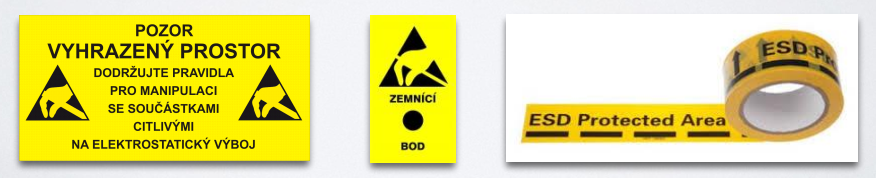
\includegraphics[scale=0.5]{images/ESD.png}
   \end{center}
   \caption{Označení ESD prostoru}
\end{figure}

\subsection{Eliminace nebezpečného náboje}
\subsubsection{Ochrana uzemněním}
Nejúčinnější ochrana před ESD spočívá v přivedení všech ESD ochranných prostředků
a personálu na stejný potenciál blížící se nule.

Nevodivé materiály a konstrukce v EPA nemohou ztratit svůj náboj uzemněním (nutno
ošetřit jiným způsobem).

Propojením všech částí pracovní oblasti na společný uzemňovací svorku (EBP -
EPA Grounding Point) prostoru EPA (pracovní plocha, podlaha, zařízení, obsluha
atp.).

Uzemňovací svorka se poté propojí se zemnící svorkou zařízení, nebo se
zemněním síťového přívodu nízkého napětí, na kterou jsou všechny pomocné
zemniče zpravidla již připojeny (vodovodní potrubí, vodivé konstrukce budovy,
regály).

\textbf{Uzemnění osob:}\\
Lidé jsou prvotními generátory statického náboje (chůze, pohyby při výrobě,
manipulaci a opravách).\\
Podmínkou je trvalé a kvalitní spojení se zemí (doporučuje se denní testování,
nebo trvalé monitorování)

\textbf{Uzemnění osob - Náramky:}\\
Hlavní ochranou pro osoby, zajišťují bezpečné převedení,
nebo rozptýlení statického náboje do země jsou náramky.\\
Náramek je podle normy vyžadován pro operace, kde
pracovníci při manipulaci nebo zpracování předmětů a
komponent citlivých na ESD sedí. Jsou tvořeny manžetou kolem zápěstí (zemnící kablík, standardně s odporem 1 M$\Omega$, 0.25 W, 250 V).

\textbf{Uzemnění osob - Sedadla:}\\
V případě lidské chyby, poruchy přístroje nebo špatného
návrhu může sedadlo poskytnout důležité rezistivní spojení
se zemí.\\
Sedadla můžou v případě nouze sloužit jako nouzové
pracovní povrchy nebo skladovací prostory (nedoporučováno v případě, že nejsou všechny sedadla antistatická)\\

\textbf{Uzemnění osob - Vozíky:}\\
Pro zajištění spojení vozíků se zemí se používají dva způsoby:\\
Elektrostaticky vodivé řetězy (nutnost zajištění dostatečně
kvalitního spojení se zemí)\\
Vodivá kola (alespoň dvě kola vozíku by měla zajišťovat
spojení se zemí)\\

\textbf{Oděvy:}\\
Jedná se o vesty, trička, pláště, pokrývky hlavy, návleky na prsty a rukavice.\\
Slouží k rozptýlení statického náboje a zabraňují jeho akumulaci zvláště ve velmi
suchém prostředí a čistých prostorech.\\

\textbf{Pracoviště EPA:}\\
Typickým příkladem je pracovní stanice,která může být umístěna podle
potřeby.(např. v montáži, ve skladu na opravárenském stanovišti, přenosné
provedení pro opravy v terénu nebo v čistých prostorech)\\
Prostor musí být označen!\\
nápisy a barevné značení na zemi, včetně označení hranice, kde je vyhrazený prostor opuštěn (viz. používané symboly)\\

\textbf{IONIZÁTORY:}\\
Neutralizace náboje v místech, kde nelze provést uzemnění vodivých částí nebo neutralizace náboje na nevodivých předmětech.\\
Dodávají stejné množství kladných i záporných iontů generovaných z okolního
vzduchu.\\
Lze je použít i v čistých prostorách, kde nelze použít chemické spreje a některé
elektrostaticky ztrátové materiály.\\


\subsection{Materiály vhodné do výrobního prostředí citlivého na ESD}

Materiály s nejnižší povrchovou rezistancí $\geq$1x10\textsubscript{2}Ohm a <1x10\textsubscript{5}Ohm jsou zařazeny jako \textbf{materiály elektrostaticky vodivé (C)}. Sem patří většina kovů, tkaniny s podílem kovového vlákna, silně vodivě dotované plasty apod. Tyto materiály se používají jednak jako ochranné a stínící, ale i jako zemniče pro odvedení vzniklého náboje. Např. obalový vodivý materiál dle normy ČSN EN 61340-5-3 má hraniční hodnotu povrchové nebo objemové rezistance <1x10\textsubscript{4}Ohm.

Materiály, jejichž povrchová rezistance je $\geq$1x10\textsubscript{5}Ohm a <1x10\textsubscript{11}Ohm jsou uváděny jako \textbf{materiály elektrostaticky ztrátové – dissipativní (D)}. Do této kategorie patří většina antistaticky upravených plastů a tkanin. Např. obalový disipativní materiál dle normy ČSN EN 61340-5-3 má rozsah povrchové nebo objemové rezistance $\geq$1x10\textsubscript{4}Ohm a <1x10\textsubscript{11}Ohm.

Materiály s povrchovou rezistancí $\geq$1x10\textsubscript{11}Ohm jsou pak považovány za \textbf{materiály izolační}. Nelze je používat ani jako ochranné či stínící. Naopak jejich výskyt je třeba na pracovištích s elektrostaticky citlivými součástkami omezit na nejnižší přijatelnou míru. Sem se řadí izolanty v klasickém slova smyslu.
























